\chapter{Introduction}
\section{Generative Design}
% What is generative design? How does it work? 
Generative design is an exploratory design method that autonomously 
generates optimal designs by iteratively varying design geometry 
to meet user-defined performance metrics 
\cite{krish_practical_2011,oh_deep_2019}.
The user defines the design parameters and the generative 
design software helps the user create many solutions 
simultaneously \cite{autodesk_autodesk_2020}. 
This sometimes results in unanticipated unique solutions, that 
would have been difficult to discover using traditional methods
\cite{autodesk_autodesk_2020}.
Generative design varies the parameters of the problem definition
\cite{matejka_dream_2018}. 
At each iteration step, the design is evaluated on the 
performance metrics. 
Based on the results, the generative design algorithm changes the 
interval allowed for each design geometry variable, refining 
design constraints (problem definition) and moving towards 
designs that best meets performance metrics.

There is confusion to how generative design differs from other shape 
optimization tools. 
Generative design is more than topology optimization which has been 
around since 1988 \cite{bendsoe_generating_1988}. 
Topology optimization requires the user to start with a complete design 
and the software improves it by removing material, it answers the 
fundamental engineering question of how to place material in a domain space 
to obtain best structural performance \cite{sigmund_topology_2013}.   
Generative design does not require the user to start with a complete design, but 
instead a few design constraints. 
Table \ref{tab:compare} summarizes the differences between generative design and 
traditional design optimization tools. 

\begin{table}[!htbp]
        \caption{Comparison of generative design and traditional design optimization tools
        \cite{autodesk_fusion_2020}.}
        \label{tab:compare}
        \centering
        \doublespacing
        \small
        \begin{tabular}{p{3.7cm}|p{5.5cm}p{6cm}}
        \hline
        \textbf{Point of Comparison} & \textbf{Generative Design} & \textbf{Traditional Design Optimization Tools}  \\ \hline
        Initial input & A few design constraints & Complete design \\ 
        No. of outcomes & Generates a wide set of designs that meets design constraints & Identifies one unique design that meets constraints \\   
        Solving strategies & Uses multiple strategies to solve design problem & Mainly uses topology optimization solutions \\ \hline
        \end{tabular}
\end{table}

% How does it actually work? What models? 
\subsection{Optimization Techniques}
Multi-objective design problems inevitably require a trade off between 
desirable attributes \cite{byrne_evolving_2014,simon_sciences_2019}. 
In nuclear reactor design there are many trade offs, one example is the 
trade-off between neutron economy and fuel enrichment. 
A reactor design must have sufficient neutron economy to ensure criticality, 
but must also have a low fuel enrichment to reduce proliferation risk.
Conflicting objectives means that there is no one perfect solution, but a set
of equally optimal solutions \cite{byrne_evolving_2014}.
Multi-objective problems are difficult to optimize, such problems 
cannot be handled by classical optimization methods such as gradient 
methods, because they tend to only find the local optimum 
\cite{renner_genetic_2003} and are efficient for a narrow subset 
of problems \cite{zames_genetic_1981}. 

Evolutionary algorithms have proven to be successful 
methods to optimize multi-objective problems \cite{krish_practical_2011} as 
they can find a solution near the global optimum \cite{renner_genetic_2003}. 
The most popular evolutionary algorithms used to solve multi-objective 
problems are genetic algorithms 
\cite{byrne_evolving_2014, krish_practical_2011}. 
Genetic algorithms differ from classical optimization techniques in four ways 
\cite{zames_genetic_1981, pereira_genetic_2000}: 
\begin{enumerate}
        \item Work with each parameter's constraints, not
        the parameters themselves. 
        \item Search a population of points, not a single point. 
        \item Does not need prior knowledge about search space and conducts
        optimization process without calculating derivatives, continuity, 
        limits, etc. 
        \item Use stochastic rules, not deterministic rules. 
\end{enumerate}

\subsubsection{Genetic Algorithms}
Genetic algorithms imitate natural selection to evolve solutions 
by (1) maintaining a population of solutions, (2) allowing 
fitter solutions reproduce, and (3) letting lesser fit solutions die off, 
resulting in final solutions that are better than the previous generations 
\cite{renner_genetic_2003}. 
Genetic algorithms demand extra computational cost compared to classical 
optimization techniques. 
Due to the availability of supercomputers, the use of genetic algorithms 
has increased and its practical application has become a reality
\cite{pereira_genetic_2000}. 
Figure \ref{fig:genetic_alg} depicts the iterative process of using a genetic 
algorithm to solve a problem. 
The key part of this process is defining evaluation and termination criteria. 
Evaluation criteria refers to the performance metrics that each solution is 
measured against. 
Termination criteria refers to the range of values for each performance metric
that a solution must meet to be considered `good enough'. 
Attainment of optimum is much less important for complex systems, the goal is 
to get a good solution without sacrificing the level of performance (speed of 
code) \cite{zames_genetic_1981}. 

\begin{figure}[!htbp]
        \centering
        \begin{tikzpicture}[node distance=1.7cm]
                \tikzstyle{every node}=[font=\small]
                \node (1) [lbblock] {\textbf{Create initial population}};
                \node (2) [lbblock, below of=1] {\textbf{Evaluate initial population}};
                \node (3) [loblock, below of=2, yshift = -1.3cm] {\textbf{Create new population:} \\ 
                \begin{enumerate} \item select individuals for mating 
                                  \item create offspring by crossover 
                                  \item mutate selected individuals 
                                  \item keep selected individuals from previous generation
                                 \end{enumerate}};
                \node (4) [loblock, below of=3, yshift=-1.3cm] {\textbf{Evaluate new population}};
                \node (5) [loblock, below of=4] {\textbf{Is termination criteria satisfied?}};
                \node (6) [lbblock, below of=5] {\textbf{Best solution is returned!}};
                \draw [arrow] (1) -- (2);
                \draw [arrow] (2) -- (3);
                \draw [arrow] (3) -- (4);
                \draw [arrow] (4) -- (5);
                \draw [arrow] (5) -- node[anchor=east] {Yes} (6);
                \draw [arrow] (5) -- ([shift={(0.5cm,0cm)}]5.east)-- node[anchor=west] {no} ([shift={(0.5cm,0cm)}]3.east)--(3);
        \end{tikzpicture}
        \caption{Process of solving a problem with genetic algorithm 
        \cite{renner_genetic_2003}. When a population does not meet termination 
        criteria, a new generation is created. This occurs iteratively till the 
        termination criteria is met. }
        \label{fig:genetic_alg}
\end{figure}

Two types of genetic algorithms are typically used to solve shape 
optimization problems: parametric and cell. 
Parametric genetic algorithms optimize complex shapes by varying parametric variables
to meet the desired design performance \cite{von_buelow_paragen_2012}.
Examples of parametric variables are: diameter of a sphere, twist angle of a cylinder, 
etc.  
Optimization of aerodynamic configurations \cite{makinen_multidisciplinary_1999}, 
and truss and bridge structures \cite{raich_evolving_2000} used parametric 
genetic algorithms.
Cell genetic algorithms represent the shape of an object to be optimized in 
small subdivided rectangular domains (pixels in 2D, voxels in 3D) 
\cite{renner_genetic_2003}. 
Figure \ref{fig:cell} shows an example of cell representation. 
Cell genetic algorithms are advantageous compared to parametric genetic 
algorithms since the initial structure and topology of the object need not 
be created and is instead developed through the iterative optimization 
process \cite{renner_genetic_2003}. 
Both parametric and cell genetic algorithms will be explored for the generative 
reactor design problem. 

\begin{figure}[!htbp]
	\begin{center}
		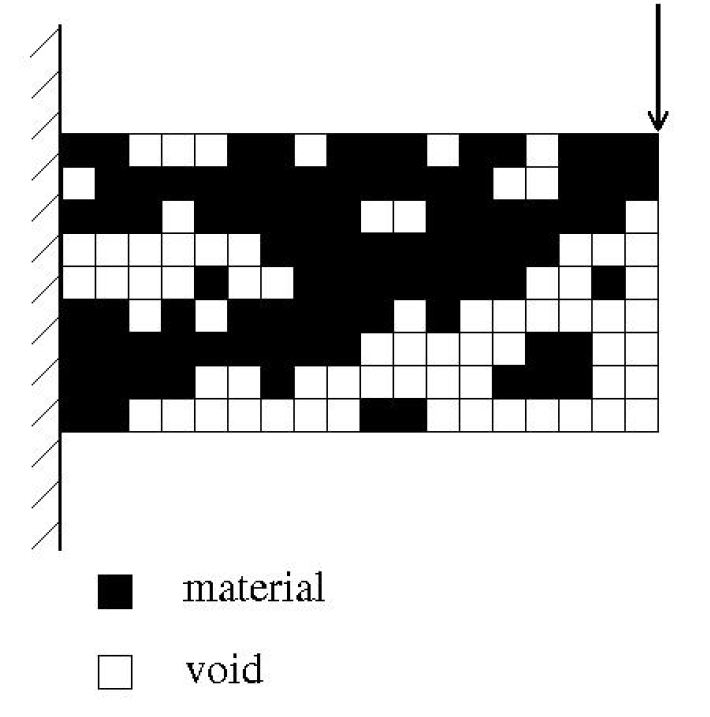
\includegraphics[scale=0.25]{./figures/cell.png}
        \end{center}	
        \caption{Cell representation in 2D \cite{renner_genetic_2003}.}
        \label{fig:cell}
\end{figure}

\subsection{State of Work}
Generative design is used in the following industries: 
automotive \cite{deplazes_autodesk_2019}, aerospace \cite{byrne_evolving_2014},
architecture, civil engineering, construction, product design etc. 
For the automotive and aerospace industries, the goal of generative 
design is to decrease 
the weight of the vehicle while ensuring each part can continue to 
withstand the stresses and strains that are put on it within a 
safety factor. 
These industries can rely on commerical softwares such as 
Autodesk Fusion360 \cite{autodesk_autodesk_2020} and  
SolidWorks Topology \cite{lombard_solidworks_2008}
to produce their generative designs, since these softwares have 
structural simulation-based generative design technology.  

Civil engineering and architecture generative design projects use specific s

\section{Generative Reactor Design}
For nuclear reactors, generative design is constrained by 
variables such as mass or volume of fuel, fuel enrichment, effectiveness 
of heat transfer, effective neutron multiplication factor, etc. 
Nuclear reactors not only experience physical forces, but also
require evaluation of the neutronics of the system, therefore generative design of 
a nuclear reactor cannot make use of tools such as Autodesk Fusion360 or SolidWorks 
Topology. 
Therefore, a framework that couples well-developed advanced genetic algorithms 
with well-supported monte-carlo particle transport 
codes (Serpent \cite{leppanen_serpent_2014}, 
MCNP \cite{werner_mcnp6._2018}, etc.) and thermal hydraulics 
codes (RELAP7 \cite{andrs_relap-7_2012} etc.)
must be created to successfully produce generative reactor designs. 

Cacuci \cite{cacuci_global_1990} has previously applied global optimization 
to the field of nuclear reactor design. 
Genetic algorithms have also been successfully applied to nuclear core reload optimization
\cite{dechaine_nuclear_1995,chapot_new_1999,schirru_genetic_1997,feltus_incorporating_1997}, 
transient classification \cite{alvarenga_adaptive_1997, mol_neural_2006}, 
core designs \cite{pereira_basic_1999,kumar_new_2015}, 
\gls{SNF} solvent extraction process 
\cite{omori_applications_1997}, design of a Fast Neutron Source (FNS) 
\cite{pevey_genetic_2019}, and finding optimized cutting paths for nuclear 
reactor decommissioning \cite{tsai_computer_2019}.  
Kumar et al \cite{kumar_new_2015} used genetic algorithms with reduced order models 
of neutronics and thermal hydraulics of the reactor to predict output parameters 
for the inputs generated by the genetic algorithm, resulting in reduced computational 
cost. 

All applications using genetic algorithms for reactor core optimization 
have varied the parameters in classical reactor geometries such as radius of 
fuel pellet and clad, enrichment of fuel, pin pitch, etc. 
Therefore, choosing parametric genetic algorithms over cell algorithms. 
In recent years, additive manufacturing technology has advanced and has altered 
the way in which components are designed and manufactured 
\cite{simpson_considerations_2019}. 
Key additive manufacturing technologies relevant to nuclear reactor 
core structures are \gls{SLM}, \gls{EBM}, and \gls{L-DED}.
The \gls{SLM} and \gls{EBM} techniques have been used for 
automotive and aircraft component fabrication \cite{murr_frontiers_2016}. 
Successful examples of additive manufacturing applied in the the aircraft industry
are Boeing's use of additive manufacturing to reduce weight in the 787 Dreamliner
\cite{noauthor_printed_2017} and SES-15 spacecraft \cite{noauthor_boeing_nodate}. 
Using additive manufacturing to fabricate nuclear reactor components will 
drastically reduce cost, timelines, increase safety and performance by tailoring 
local material properties and redesigning geometries for optimal load paths 
\cite{simpson_considerations_2019}. 
With further advancement of these additive manufacturing technologies, 
a reactor core could be 3D printed in the near future. 
Therefore, with the capability to 3D print a nuclear reactor, genetic algorithms 
can be leveraged to optimize the reactor core in non-classical ways, such as wavy
coolant channels and spatially-variant optimized packing of \gls{TRISO} particles, 
etc.  
% cite pre application narrative? 


\subsection{Workflow}
% How the genetic algorithm is coupled with a CAD designer and analysis tool 
% (serpent/RELAP)
% CAD designer > grasshopper3d (see Bryne Paper)
Figure \ref{fig:workflow} depicts a framework for leveraging genetic algorithms
to design nuclear reactors. 
This is a general framework that does not specify algorithms or analytical 
softwares. 
Instead, it provides placeholders for algorithm and software types, so 
that a user may choose the types of algorithms and softwares they want to use in 
their mission towards using generative design to design a nuclear reactor. 
Table \ref{tab:examples} lists algorithm and software types that could be used 
in the framework. 

\begin{figure}[!htbp]
        \centering
        \begin{tikzpicture}[node distance=2cm]
                \tikzstyle{every node}=[font=\small]
                \node[anchor=west] (1) [noblock] {\textbf{Create}};
                \node (2) [bblock, right=of 1] {\textbf{GA: Creates population}};
                \node (3) [pblock, right=of 2] {\textbf{GGS: Generates reactor designs}};
                \node[anchor=west] (4) [noblock, below of= 1] {\textbf{Analyze}};
                \node (5) [oblock, below of =2]{\textbf{NT: Run NT code for each solution}};
                \node (6) [gblock, right=of 5]{\textbf{TH: Run TH code for each solution}};
                \node[anchor=west] (7) [noblock, below of= 4] {\textbf{Evaluate}};
                \node (8) [bblock, below of =5] {\textbf{GA: Evaluate population}};
                \node (9) [ppblock, right=of 8] {\textbf{M: Evaluation based on performance metrics}};
                \node[anchor=west] (10) [noblock, below of= 7] {\textbf{Check}};
                \node (11) [lppblock, below of=8, xshift=3cm, yshift=-0.2cm] {\textbf{M: Is termination criteria met?}};
                \node (16) [lbblock, below of = 11] {\textbf{GA: Best solution is returned!}};
                \node[anchor=west] (12) [snoblock, above of= 2, xshift=3cm, yshift=-1.1cm] {};
                \node[anchor=west] (13) [snoblock, below of=12,yshift=-0.15cm] {};
                \node[anchor=west] (14) [snoblock, below of=13,yshift=-0.02cm] {};
                \node[anchor=west] (15) [snoblock, below of=14,yshift=-0.02cm] {};
                \node[anchor=west] (17) [noblock, below of= 10] {\textbf{Completed}};
                \draw [-,thick] (11) -- ([shift={(3cm,0cm)}]11.east) |- node[anchor=west, yshift=-4.2cm] {no} ([shift={(0cm,0.7cm)}]12.north)--(12);
                \draw [arrow] (12) -- ([shift={(0cm,0cm)}]12.north) |- ([shift={(0cm,0.4cm)}]2.north)--(2);
                \draw [arrow] (12) -- ([shift={(0cm,0cm)}]12.north) |- ([shift={(0cm,0.4cm)}]3.north)--(3);
                \draw [-,thick] (2) -- ([shift={(0cm,0cm)}]2.south) |- ([shift={(0cm,0.3cm)}]13.north)--(13);
                \draw [-,thick] (3) -- ([shift={(0cm,0cm)}]3.south) |- ([shift={(0cm,0.3cm)}]13.north)--(13);
                \draw [arrow] (13) -- ([shift={(0cm,0cm)}]13.north) |- ([shift={(0cm,0.3cm)}]5.north)--(5);
                \draw [arrow] (13) -- ([shift={(0cm,0cm)}]13.north) |- ([shift={(0cm,0.3cm)}]6.north)--(6);
                \draw [-,thick] (5) -- ([shift={(0cm,0cm)}]5.south) |- ([shift={(0cm,0.3cm)}]14.north)--(14);
                \draw [-,thick] (6) -- ([shift={(0cm,0cm)}]6.south) |- ([shift={(0cm,0.3cm)}]14.north)--(14);
                \draw [arrow] (14) -- ([shift={(0cm,0cm)}]14.north) |- ([shift={(0cm,0.3cm)}]8.north)--(8);
                \draw [arrow] (14) -- ([shift={(0cm,0cm)}]14.north) |- ([shift={(0cm,0.21cm)}]9.north)--(9);
                \draw [-,thick] (8) -- ([shift={(0cm,0cm)}]8.south) |- ([shift={(0cm,0.3cm)}]15.north)--(15);
                \draw [-,thick] (9) -- ([shift={(0cm,0cm)}]9.south) |- ([shift={(0cm,0.3cm)}]15.north)--(15);
                \draw [arrow] (15) -- ([shift={(0cm,0cm)}]15.north) |- ([shift={(0cm,0.1cm)}]11.north)--(11);
                \draw [arrow] (11) -- ([shift={(0cm,0cm)}]11.south) |- node[anchor=west, yshift=0.3cm] {yes} ([shift={(0cm,0.1cm)}]16.north)--(16);
                \matrix [draw,below left,yshift=-0.5cm, xshift=-7cm] at (current bounding box.south east) {
                \node [bbblock,label=right:\textbf{GA: Genetic algorithm}] {}; \\
                \node [bpblock,label=right:\textbf{GGS: Geometry generating software}] {}; \\
                \node [boblock,label=right:\textbf{NT: Neutron transport code}] {}; \\
                \node [bgblock,label=right:\textbf{TH: Thermal hydaulics code}] {}; \\
                \node [bppblock,label=right:\textbf{M: User-defined metrics/criteria}] {}; \\
                };
        \end{tikzpicture}
        \caption{Generative reactor design framework. Each component of the 
        framework is user-selected.}
        \label{fig:workflow}
\end{figure}

\begin{table}[!htbp]
        \caption{Example algorithm and software types to populate generative reactor 
        design framework (Fig \ref{fig:workflow}).}
        \label{tab:examples}
        \centering
        \doublespacing
        \small
        \begin{tabular}{lp{10cm}}
        \hline
        \textbf{Framework Component} & \textbf{Examples}\\ \hline
        Genetic algorithm driver & DEAP \cite{fortin_deap_2012} \\
        Geometry generating software & Trelis \cite{noauthor_trelis_2018}, FreeCAD \cite{falck_freecad_2012}, SolidWorks \cite{lombard_solidworks_2008}, grasshopper3d \cite{rutten_grasshopper3d_2015}, GenerativeComponents \cite{aish_bentleys_2003}, Trilinos \cite{heroux_overview_2003}, DAGMC \cite{smith_enhanced_2011} \\
        Neutron transport code & Serpent \cite{leppanen_serpent_2014}, MCNP \cite{werner_mcnp6._2018}, SCALE \cite{bucholz_scale:_1982}, OpenMC \cite{romano_openmc_2013} \\ 
        Thermal hydraulics code & RELAP5-3D \cite{strydom_comparison_2016}, RELAP7 \cite{andrs_relap-7_2012}, TRACE \cite{xu_multi-physics_2006}\\
        User-defined metrics/criteria & keff, heat transfer rate, fuel enrichment, mass of fuel \\ \hline
\end{tabular}
\end{table}

\subsection{Software}
The generative reactor design framework proposed (Fig. \ref{fig:workflow}) 
has many coupled components. 
To minimize the amount of coupling required, software is chosen with 
framework-leanness in mind. 
The shortlisted software will be evaluated based on the clearly 
defined requirements of each component. 
Each iteration of the framework requires the neutron transport code, 
the thermal hydraulics code, and evaluation to be run for each 
nuclear reactor geometry (individual) generated by the genetic algorithm, 
resulting in a high computational cost. 
Since each individual can be evaluated independently from others, 
individual runs must be parallelized to reduce computation time 
\cite{pereira_genetic_2000}. 
The generative reactor design framework is computation-heavy. 
To produce results in a timely manner, a supercomputer 
such as Blue Waters \cite{ncsa_about_2017} will be used. 
In summary, each component's software is chosen based on these 
conditions: 
\begin{enumerate}
    \item It best meets the clearly defined requirements 
    its respective component. 
    \item It is parallelizable. 
    \item It is compatible with a high performance computer. 
    \item It is open-source and free (preferable but not required). 
\end{enumerate}

The subsequent subsections will define the requirements of each 
component in the generative reactor framework, the software considered, 
and an explanation justifying the final software choice. 

\subsubsection{Genetic Algorithm Driver}
Evolutionary algorithm computation is a sophisticated field with diverse
techniques and mechanisms, resulting in even well designed frameworks 
being complicated under the hood \cite{fortin_deap_2012}. 
These implementation intricacies are difficult to extend since it requires 
the user to edit the source code. 
This is concerning since using evolutionary algorithms to solve unique 
real-world problems requires customization of algorithms 
\cite{fortin_deap_2012}. 
Therefore, an evolutionary algorithm computation framework that gives 
the user the capability to build custom evolutionary algorithms is 
required for this project. 

There are many evolutionary algorithm computation packages 
available: \gls{DEAP} \cite{fortin_deap_2012}, 
inspyred \cite{garrett_inspyred_2014}, 
Pyevolve \cite{perone_pyevolve_2009}, and
OpenBEAGLE \cite{gagne_open_2002}. 
DEAP is the most newly created package and places a high value on 
code compactness and code clarity \cite{fortin_deap_2012}. 
\gls{DEAP} is the only framework that allows the user to rapidly 
prototype evolutionary algorithms and define custom algorithms without 
having to dig deep into the source code to modify lines, making it 
the code of choice for the genetic algorithm driver component of 
the generative reactor design framework. 
\gls{DEAP} provides building blocks for each optimizer function and 
allows the user to customize and design a specialized algorithm 
to fit their project. 

\subsubsection{Geometry Generating Software}
The geometry generating software is the `filling' in the sandwich in which 
the top bun is the genetic algorithm driver and bottom bun is the 
analysis codes (neutron transport and thermal hydraulics). 
The geometry generating software must easily interface with the
\gls{DEAP} genetic algorithm driver by accepting Python scripting commands to 
generate 3D geometries. 
The geometry generating software must be compatible with file formats 
accepted by the analysis codes. 
Serpent neutron transport code accepts STL and OpenFOAM file formats. 
The geometry generating software must be easily controlled from the command line
to generate geometries without needing to open a \gls{GUI}, enabling its use 
on a supercomputer. 

\subsubsection{Neutron Transport Code}
Many neutron transport codes have restricted public access. 
In this project, the Serpent Monte Carlo code is used. 
The reasons for choosing Serpent are: 
\begin{itemize}
    \item It is designed to be parallelizable on high performance 
    computers. 
    \item It is already installed on the Blue Waters supercomputer at UIUC. 
    \item UIUC has gained access to the Serpent code through RSICC. 
\end{itemize}

\subsubsection{Thermal Hydraulics Code}

\subsection{Metrics}

\subsubsection{Performance Metrics}
Table \ref{tab:eval-metric} describes the performance metrics that each 
reactor geometry will be evaluated against. 
Based on how `well' each reactor geometry does for each evaluation metric, 
a fitness value is calculated to determine if the reactor geometry is good 
enough to be used to generate the next population of reactor geometries. 

\begin{table}[!htbp]
    \caption{Performance Metrics for each reactor geometry.}
    \label{tab:eval-metric}
    \centering
    \doublespacing
    \small
    \begin{tabular}{ll}
    \hline
    \textbf{Categories} & \textbf{Evaluation Metrics}\\ \hline
    & Maximize power [$\frac{MW}{g}$] \\
    Neutron Transport & Full core \gls{PPF}, Assembly \gls{PPF} \\ 
    & keff $\sim$ 1 \\ 
    & Minimize fuel amount [kg] \\ \hline
    Thermal Hydraulics & Maximize surface area for heat transfer [$m^2$]\\ 
    & Minimize pressure drop [Pa]\\ \hline 
    \end{tabular}
\end{table}

Power peaking factor is highest \gls{LPD} divided by average power density in 
the reactor core. 

\subsubsection{Termination Criteria}
The termination criteria is met when all evaluation metrics converge. 

\section{\gls{FHR}}
For this project, generative reactor design is explored for the 
\gls{FHR}. 
The \gls{FHR} is a reactor concept introduced in 2012 that uses high-temperature 
coated-particle fuel and a low pressure liquid fluoride-salt coolant 
\cite{forsberg_fluoride-salt-cooled_2012,facilitators_fluoride-salt-cooled_2013}.
\gls{FHR} technology combines the best aspects of \gls{MSR} and\gls{HTGR} 
technologies. 
Molten fluoride salts as working fluids for nuclear reactors have been explored 
since the 1960s and are desirable because of the salts' high-temperature 
performance and overall chemical stability \cite{scarlat_design_2014}.  
Using molten salts for reactor coolant introduces inherent safety compared 
to water due to the salts' high boiling temperature and high volumetric 
heat capacity, eliminating the risk of coolant boiling off, resulting in 
fuel elements overheating \cite{ho_molten_2013}. 
The leading candidate coolant salt is the fluoride salt Li$_2$BeF$_4$ (FLiBe), 
which remains liquid without pressurization up to 1400$\degree$C and a larger 
$\rho C_p$ than water \cite{ho_molten_2013,forsberg_fluoride-salt-cooled_2012}. 
\glspl{FHR} are favorable compared to a liquid fuel reactor because the solid 
fuel cladding adds an extra barrier to fission product release 
\cite{ho_molten_2013}.
\gls{HTGR} technology has been studied since the 1970s because it delivers 
heat at substantially high temperatures than \glspl{LWR} resulting in 
the following advantages: increased power conversion efficiency, reduced 
waste heat generation, and co-generation and process heat capabilities 
\cite{scarlat_design_2014}. 
In \glspl{HTGR}, the helium coolant is held at a high pressure of approximately 
100 atm, while \gls{FHR}'s FLiBe coolant is at room pressure, resulting in lower 
construction costs since a thick concrete reactor vessel is not required.
The molten salt coolant has superior cooling and moderating properties compared 
to helium coolant in \glspl{HTGR}, resulting in \glspl{FHR} operating at 
power densities two to six times higher than  \glspl{HTGR} 
\cite{scarlat_design_2014,forsberg_fluoride-salt-cooled_2012}.
Therefore, by combining the FLiBE coolant from \gls{MSR} technology and 
\gls{TRISO} particles from \gls{HTGR} technology, the \gls{FHR} benefits from 
the low operating pressure and large thermal margin provided by using a molten 
salt coolant and the accident-tolerant qualities of \gls{TRISO} particle fuel. 

There are several types of \gls{FHR} designs that are being developed worldwide: 
circulating pebbles (\gls{PBFHR}, Kairos Power Reactor) and hexagonal fuel plate elements (\gls{AHTR}). 

% Benchmark? 

\subsection{Modelling Challenges}
% why is it so hard to model a FHR
Verification and validation of a simulation tool is a crucial step to successfully 
model a reactor with the goal of deployment \cite{rahnema_phenomena_2019}. 
The \gls{FHR} has a complex core design due to the multiple heterogeneity present 
in the fuel introduced by presence of \gls{TRISO} particles and other moderating 
materials (i.e.in the \gls{AHTR}, \gls{TRISO} particles pressed into plates, which 
are bundled into assembles) \cite{ramey_monte_2018,rahnema_phenomena_2019}.
Traditional homogenization methods are insufficient to capture the correct physics 
in \glspl{FHR}, due to the multiple heterogeneity \cite{ramey_monte_2018}. 
For example, in the \gls{PBFHR}, pebble packing variation effects are significant, 
resulting in large errors at the outer edge of the core when homogenized 
\cite{rahnema_phenomena_2019}. 
In the \gls{AHTR}, single and multiple slab homogenization decreased computation time 
by 10, however they introduce a nontrivial error of $\sim$3\%
\cite{ramey_monte_2018,cisneros_neutronics_2012}.
% random stuff to take note of 
Both full core peaking factor and within-assembly peaking factor must be evaluated, 
due to the non-uniformity in fission density of individual \gls{TRISO} particles. 
Neutron spectra in different materials and regions must be investigated and compared 
against assembly averaged spectra. 
The \gls{FHR} consists of materials that are known to have uncertainty 
in nuclear cross-section data such as the moderation, thermalization, and absorption 
for FliBE constituents and the thermalization and absorption 
in the carbon within the graphite matrix \cite{rahnema_phenomena_2019}. 
 
\subsection{Previous \gls{FHR} Modeling and Simulation Efforts}
% Previous efforts to model each type of FHR. Plate & Pebble  
Ramey et al \cite{ramey_monte_2018} conducted a 2D \gls{AHTR} assembly model with 
continuous energy cross sections in SERPENT (\gls{TRISO}-level results were also 
included). 
Zhang et al introduced a 3D \gls{AHTR} benchmark \cite{zhang_stylized_2018}
and solved it using the continuous-energy COMET code 
\cite{zhang_continuous-energy_2018}. 
The COMET solution was in good agreement with the \gls{MCNP} reference solutions
\cite{zhang_continuous-energy_2018}. 



